% ============================================================
% main.tex
% Digital Innovation — Written Case Solution
% SDC / AAUBS / UCAS · 2026
% ============================================================
% This is the master file. It pulls in the preamble, macros,
% and one file per section. Compile with:
%
%   pdflatex main.tex
%   biber main
%   pdflatex main.tex
%   pdflatex main.tex
%
% In Overleaf this happens automatically when you click
% Recompile. If you see missing references or bibliography
% errors, click the dropdown next to Recompile and choose
% "Recompile from scratch."
% ============================================================

% ============================================================
% NOTE: Do not compile this file directly. Compile main.tex instead.
% ============================================================
% preamble.tex
% Digital Innovation — Hand-in Template
% SDC / AAUBS / UCAS · 2026
% Eskil Olav Andersen, Aalborg University Business School
% ============================================================
% This preamble is intentionally readable. Change what you
% need; leave comments so your group knows what each block does.
% ============================================================

\documentclass[12pt, a4paper]{article}

% ── Encoding and language ────────────────────────────────────
\usepackage[utf8]{inputenc}
\usepackage[T1]{fontenc}
\usepackage[english]{babel}
\usepackage{csquotes}           % required by biblatex
\usepackage{algorithm}
\usepackage{algorithmic}
\usepackage{tikz}

% ── Fonts ────────────────────────────────────────────────────
% Lato is the AAU brand font. If it is unavailable in your
% LaTeX distribution, remove these two lines — the document
% will fall back to the default sans-serif font.
\usepackage{lato}
\renewcommand{\familydefault}{\sfdefault}

% ── Page geometry ────────────────────────────────────────────
% Standard margins for a 10-page report. Adjust if needed.
\usepackage[
  a4paper,
  top=25mm,
  bottom=25mm,
  left=30mm,
  right=25mm,
  headheight=25pt
]{geometry}

% ── AAU color palette ────────────────────────────────────────
% These match the slide deck exactly. Use them via the named
% shortcuts defined in macros.tex rather than raw RGB values.
\usepackage{xcolor}

\definecolor{aaublue}{RGB}{31, 25, 82}           % AAU deep navy
\definecolor{aaulightblue}{RGB}{64, 102, 178}    % AAU mid blue
\definecolor{aaugray}{RGB}{67, 90, 105}          % AAU gray
\definecolor{aaulightgray}{RGB}{166, 168, 171}   % AAU light gray
\definecolor{aausilver}{RGB}{237, 237, 237}      % AAU silver background
\definecolor{aauorange}{RGB}{187, 91, 24}        % AAU orange (accent)
\definecolor{aaugreen}{RGB}{15, 134, 98}         % AAU green
\definecolor{aaured}{RGB}{204, 68, 92}           % AAU red

\colorlet{primarycolor}{aaublue}
\colorlet{accentcolor}{aauorange}

% ── Core packages ────────────────────────────────────────────
\usepackage{graphicx}           % figures
\usepackage{booktabs}           % professional tables
\usepackage{array}
\usepackage{multirow}
\usepackage{microtype}          % better text spacing
\usepackage{parskip}            % paragraph spacing instead of indent
\usepackage{setspace}
\setstretch{1.15}

% ── Mathematics ──────────────────────────────────────────────
\usepackage{amsmath}            % equations, align, etc.
\usepackage{amssymb}            % \mathbb, \mathcal, etc.

% ── Callout boxes ────────────────────────────────────────────
\usepackage{tcolorbox}
\tcbuselibrary{skins, breakable}

% ── Headers and footers ──────────────────────────────────────
\usepackage{fancyhdr}
\pagestyle{fancy}
\fancyhf{}
\fancyhead[L]{\small\textcolor{aaugray}{Digital Innovation · SDC / AAUBS / UCAS · 2026}}
\fancyhead[R]{}
\fancyfoot[C]{\small\textcolor{aaugray}{\thepage}}
\renewcommand{\headrulewidth}{0.4pt}
\renewcommand{\headrule}{\hbox to\headwidth{\color{primarycolor}\leaders\hrule height \headrulewidth\hfill}}

% ── Section heading style ────────────────────────────────────
% Clean, navy headings. Adjust font sizes to your preference.
\usepackage{titlesec}
\titleformat{\section}
  {\large\bfseries\color{primarycolor}}
  {\thesection.}{0.6em}{}
  [\vspace{-0.3em}\textcolor{primarycolor!30}{\rule{\linewidth}{0.4pt}}]

\titleformat{\subsection}
  {\normalsize\bfseries\color{primarycolor}}
  {\thesubsection}{0.5em}{}

% Unnumbered subsections inherit the subsection style above.

% ── TikZ and diagrams ────────────────────────────────────────
% Used in the appendix architecture diagram example.
% Safe to remove if you are not drawing diagrams.
\usepackage{tikz}
\usetikzlibrary{arrows.meta, shapes.geometric, shapes,
                positioning, calc, backgrounds, fit}

% ── Hyperlinks ───────────────────────────────────────────────
\usepackage{hyperref}
\hypersetup{
  colorlinks  = true,
  linkcolor   = primarycolor,
  urlcolor    = primarycolor,
  citecolor   = primarycolor,
  filecolor   = primarycolor,
  pdftitle    = {Digital Innovation — Case Solution},
  pdfauthor   = {Student Team},
}

% ── Bibliography ─────────────────────────────────────────────
% APA style as required. Biber is the recommended backend.
% Compile order: pdflatex → biber → pdflatex → pdflatex
\usepackage[style=apa, backend=biber]{biblatex}
\addbibresource{bib/references.bib}

% ============================================================
% macros.tex
% Digital Innovation — Hand-in Template
% SDC / AAUBS / UCAS · 2026
% Eskil Olav Andersen, Aalborg University Business School
% ============================================================
% A lean set of reusable commands. The principle: define only
% what genuinely recurs. Add your own at the bottom following
% the same pattern. Delete anything you do not use.
% ============================================================

\usepackage{xspace}

% ── Institutional shorthands ─────────────────────────────────
% Saves typing and keeps spelling consistent throughout.
%
%   \aaubs    →  Aalborg University Business School  (navy bold)
%   \sdc      →  Sino-Danish Center                  (navy bold)
%   \ucas     →  UCAS                                (navy bold)
%   \ai       →  AI                                  (navy bold)
%   \genai    →  GenAI                               (navy bold)

\newcommand{\aaubs}{\textbf{\color{primarycolor}Aalborg University Business School}\xspace}
\newcommand{\sdc}{\textbf{\color{primarycolor}Sino-Danish Center}\xspace}
\newcommand{\ucas}{\textbf{\color{primarycolor}UCAS}\xspace}
\newcommand{\ai}{\textbf{\color{primarycolor}AI}\xspace}
\newcommand{\genai}{\textbf{\color{primarycolor}GenAI}\xspace}

% ── Typography utilities ─────────────────────────────────────

% \keyterm{text}
% First introduction of a concept — navy bold.
% Use once per term, not as general emphasis.
% Example: \keyterm{Technology-Organization-Environment (TOE) framework}
\newcommand{\keyterm}[1]{\textbf{\color{primarycolor}#1}}

% \highlight{text}
% Inline accent highlight — orange background, bold.
% Use at most once or twice per page. Loses effect if overused.
% Example: \highlight{binding constraint}
\newcommand{\highlight}[1]{\colorbox{accentcolor!20}{\textbf{#1}}}

% \source{attribution}
% Unobtrusive source line — sits below a figure or table.
% Example: \source{Tornatzky \& Fleischer, 1990}
\newcommand{\source}[1]{%
  \begin{flushright}
    \footnotesize\textit{\color{aaugray}Source: #1}
  \end{flushright}%
}

% \tocite
% Placeholder for a citation you still need to fill in.
% Shows [CITE] in orange so it is visible during drafting.
% Replace every instance before submission.
% Example: The model performed well in early tests \tocite.
\newcommand{\tocite}{\textcolor{accentcolor}{\textbf{[CITE]}}\xspace}

% ── Research question box ────────────────────────────────────
%
% \rqbox{Your research question here.}
%
% A prominent display box for your guiding research question.
% Use once, in the introduction. The box signals to the reader
% that everything that follows is organized around this question.
%
% Example:
%   \rqbox{What stands between our replenishment tool and
%   adoption by an independent pharmacy, and what did
%   building it teach us about working with AI?}
%
% You can modify the colors by changing primarycolor and
% accentcolor!40 below to any color defined in preamble.tex.

\newcommand{\rqbox}[1]{%
  \begin{tcolorbox}[
    enhanced,
    colback    = primarycolor!5,
    colframe   = primarycolor,
    leftrule   = 4pt,
    rightrule  = 0.4pt,
    toprule    = 0.4pt,
    bottomrule = 0.4pt,
    arc        = 2pt,
    left       = 10pt,
    right      = 10pt,
    top        = 8pt,
    bottom     = 8pt,
    fonttitle  = \small\bfseries\color{primarycolor},
    title      = {Guiding Research Question},
  ]
  \small\itshape #1
  \end{tcolorbox}%
}

% ── General callout / insight box ────────────────────────────
%
% \insightbox[color]{Label}{Content}
%
% A flexible box for key findings, limitations, or takeaways.
% The optional color argument defaults to primarycolor.
% The label appears as a bold title inside the box.
%
% Examples:
%   \insightbox{Key finding}{The binding constraint is not
%   technical readiness but organizational capacity to
%   interpret AI output without supplementary lookup.}
%
%   \insightbox[aaugreen]{Confirmed}{Output quality met the
%   threshold for user trust within the first session.}
%
%   \insightbox[aaured]{Limitation}{The model has no access
%   to live pricing data; all outputs reflect a static
%   snapshot from the training period.}

\newcommand{\insightbox}[3][primarycolor]{%
  \begin{tcolorbox}[
    enhanced,
    colback    = #1!6,
    colframe   = #1,
    leftrule   = 4pt,
    rightrule  = 0.4pt,
    toprule    = 0.4pt,
    bottomrule = 0.4pt,
    arc        = 2pt,
    left       = 10pt,
    right      = 10pt,
    top        = 7pt,
    bottom     = 7pt,
    fonttitle  = \small\bfseries\color{#1},
    title      = {#2},
    breakable,
  ]
  \small #3
  \end{tcolorbox}%
}

% ── Add your own macros below ────────────────────────────────
% Follow the same pattern: a short comment, the definition,
% and at least one usage example in a comment.
%
% Example of a simple shorthand:
%   \newcommand{\productname}{ReplenishAI\xspace}
%   % Usage: \productname is a forecasting tool for ...


% ============================================================
% Document metadata
% Fill in your group's details here.
% ============================================================

\newcommand{\ProductName}{Maverick-SORT}
\newcommand{\CaseName}{Pharmaceutical Distribution Warehouse Wave Allocation}
\newcommand{\GroupMembers}{Junyuan Luo}
\newcommand{\SubmissionDate}{12 June 2026}

% ============================================================
\begin{document}
% ============================================================

% ── Title page ───────────────────────────────────────────────
% The title page uses TikZ for the header and footer bars
% (matching the visual identity of the slide deck) and
% \includegraphics for the institution logos.
%
% To restyle: change the fill colors, adjust logo heights,
% or replace the bar-based design entirely. The page uses
% \thispagestyle{empty} so the header/footer from fancyhdr
% does not appear on top of the custom design.

\begin{titlepage}
\thispagestyle{empty}

\begin{tikzpicture}[remember picture, overlay]
  % Top bar — primary navy
  \fill[primarycolor]
    (current page.north west) rectangle
    ([yshift=-1.2cm] current page.north east);

  % Bottom bar — accent orange
  \fill[accentcolor]
    ([yshift=1.0cm] current page.south west) rectangle
    (current page.south east);

  % AAUBS2 wordmark — top right inside bar
  % Placed on a small white pill so it is legible on the navy bar.
  \node[anchor=east] at
  ([xshift=-1.2cm, yshift=-0.6cm] current page.north east) {
    \colorbox{primarycolor}{%
      \color{white}%
      
\includegraphics[height=0.6cm]{media/images/AAUBS2white.png}%
    }
  };
\end{tikzpicture}

% ── Title block ──────────────────────────────────────────────
\vfill

\begin{center}

  {\footnotesize\textcolor{aaugray}{\MakeUppercase{Digital Innovation · Module 2.4}}}\\[0.4em]
  {\footnotesize\textcolor{aaugray}{SDC / AAUBS / UCAS · 2026}}

  \vspace{1.6cm}

  {\LARGE\bfseries\color{primarycolor} \ProductName}

  \vspace{0.6em}

  {\large\textcolor{aaugray}{\CaseName}}

  \vspace{0.5em}
  \textcolor{primarycolor!30}{\rule{0.4\linewidth}{0.8pt}}

  \vspace{1.6cm}

  {\normalsize\textcolor{aaugray}{\GroupMembers}}

  \vspace{0.8cm}

  {\small\textcolor{aaugray}{\SubmissionDate}}

\end{center}

% ── Logo row ─────────────────────────────────────────────────
\vfill
\begin{center}
  
\includegraphics[height=1.1cm]{media/images/AAUBS.png}%
  \hspace{2.0em}%
  \textcolor{aaugray!40}{\rule{0.4pt}{1.0cm}}%
  \hspace{2.0em}%
  
\includegraphics[height=1.1cm]{media/images/SDC.png}%
  \hspace{2.0em}%
  \textcolor{aaugray!40}{\rule{0.4pt}{1.0cm}}%
  \hspace{2.0em}%
  
\includegraphics[height=1.1cm]{media/images/UCAS.png}%
\end{center}
\vfill

\end{titlepage}

% ── Table of contents ────────────────────────────────────────
% Remove or comment out if you prefer to start directly
% with Section 1. On a 10-page document a ToC is optional.
\tableofcontents
\newpage

% ============================================================
% Main sections
% Each \input pulls in one section file from sections/.
% To reorder sections: rearrange the \input lines below.
% To combine sections: merge two files or add content here.
% ============================================================

% ============================================================
% 01_problem.tex
% Section 1: Problem and Product Grounding
% ============================================================

\section{Problem and Product Grounding}

\subsection{The User and the Problem}

Based on the case offered by the professor, the main target users should be the operations director of a mid-sized pharmaceutical distribution warehouse in China, whose warehouse processes approximately 2,000 orders daily across 42,000 SKUs, with temperature requirements spanning ambient, cool, cold, and frozen categories. Every morning at 7:00 AM, the operations team will gather around a whiteboard to manually group orders into ``waves'' (batches) for coordinated picking. The rules they use are simple: group by temperature zone first, then by geographic proximity. They have done this for eight years.

The problem is that this manual process is increasingly untenable. Three forces converge:

\begin{enumerate}
    \item \textbf{SKU complexity}: 38\% of SKUs are near-expiry managed items with varying temperature requirements; cross-zone contamination risks GSP (Good Supply Practice) violations\parencite{paxafe2025ai}.
    \item \textbf{Order fragmentation}: Daily active customers exceed 1,200, mostly small-batch orders averaging 3--5 items, making manual grouping cognitively demanding.
    \item \textbf{Peak volatility}: During flu seasons and promotional periods, order volume spikes to 280\% of baseline, overwhelming the whiteboard method.
\end{enumerate}

What they need is a way to see, in five minutes, whether AI-driven wave allocation would actually save their money---before they commit to any integration.

\subsection{What the Product Does Today}

\textbf{Maverick-SORT} is a web-based decision-support tool for pharmaceutical wave allocation. It does not replace the users' existing Warehouse Management System (WMS). Instead, it sits alongside it, consuming order data and recommending wave compositions that minimize total operational cost while respecting temperature compliance and deadline constraints.

I built two versions, but the focus of this reflection is the \textbf{Essential Edition}---the version Wang Li would actually try first:

\begin{itemize}
    \item \textbf{KGDRL Core Engine}: A Knowledge-Guided Deep Reinforcement Learning algorithm that learns to allocate orders to waves, guided by pharmaceutical-domain heuristics (temperature matching, zone proximity, earliest-due-date).
    \item \textbf{Algorithm Arena}: A comparison dashboard showing how KGDRL performs against five rule-based baselines (FCFS, TEMP\_FIRST, ZONE\_NN, EDD, TZU) on metrics including picking distance, temperature violations, and deadline misses.
    \item \textbf{What-If Scenario Simulator}: A parameter-sensitivity tool that lets Wang Li ask ``What if I change wave capacity from 20 to 15?'' and see the impact on cost and service level---without touching her live system.
\end{itemize}

The product is deliberately narrow. We resisted the temptation to build a full WMS replacement, an ERP connector, or a robotic control layer. The value proposition is singular: \textit{in five minutes, know whether AI scheduling is worth your money}.

\subsection{Guiding Question}

This document asks: \textbf{What most limits Maverick-SORT from reaching real use by pharmaceutical warehouse operators, and what does building it teach us about working with AI?}

The sections that follow each help answer this question. Section~\ref{sec:architecture} describes the technical choices and their consequences. Section~\ref{sec:building} examines where we handed work to the AI agent and where our own judgment did the real work. Section~\ref{sec:theory} connects the build process and the product to course theory along two threads: AI and work, and adoption and diffusion. Section~\ref{sec:results} assesses what works, what does not, and what comes next.

\rqbox{What most limits Maverick-SORT from reaching real use by pharmaceutical warehouse operators, and what does building it teach us about working with AI?}


% ============================================================
% 02_architecture.tex
% Section 2: Technical Architecture and Choices
% ============================================================

\section{Technical Architecture and Choices}\label{sec:architecture}

\subsection{Algorithm: Knowledge-Guided Deep Reinforcement Learning}

The wave allocation problem is a sequential decision problem under uncertainty. Orders arrive stochastically over time; at each decision point, the system must either add an order to the current wave or close the wave and dispatch it for picking. We formulate this as a finite-horizon Markov Decision Process $M = (\mathcal{S}, \mathcal{A}, \mathcal{P}, \mathcal{R}, \gamma)$.

\textbf{State space} $\mathcal{S}$ encodes: (i) the current wave's composition (order count, volume, zone coverage, temperature coverage); (ii) the top-$K$ candidate orders from the pool, ranked by deadline urgency; (iii) temporal features (arrival rate, shift time remaining); and (iv) historical statistics (cumulative distance, violations).

\textbf{Action space} $\mathcal{A}$ comprises: (a) adding a specific candidate order to the active wave, or (b) closing the wave and opening a new one.

\textbf{Reward function} combines four components:
\begin{equation}
    r(s_t, a_t) = -\alpha_{\text{eff}} \cdot \Delta L - \alpha_{\text{temp}} \cdot \mathbb{1}_{[\text{violation}]} - \alpha_{\text{deadline}} \cdot \max(0, t_{\text{finish}} - d_o) - \alpha_{\text{setup}} \cdot \mathbb{1}_{[a_t = \text{CLOSE}]}
\end{equation}
where $\Delta L$ is estimated picking distance increment, and the indicator terms penalize temperature violations, deadline misses, and wave setup costs respectively.

The core algorithmic contribution is the \textbf{KGDRL architecture}, which integrates three mechanisms:

\begin{enumerate}
    \item \textbf{Graph Attention Network (GAT) encoder}: The state is represented as a heterogeneous graph with nodes for orders, zones, temperature categories, and the current wave. A two-layer GAT learns attention-weighted embeddings that capture spatial and thermal relationships\parencite{liu2024dynamic, sun2024gat}.
    \item \textbf{Knowledge injection via KL divergence}: A pre-trained heuristic (TZU: Temperature-Zone-Urgency) generates demonstration trajectories. During PPO training, a KL-divergence term $D_{\text{KL}}(\pi_\theta \| \pi_{\text{TZU}})$ constrains the policy to stay close to domain expertise, ensuring GSP-compliance rules are not forgotten during exploration.
    \item \textbf{Behavioral cloning pre-training}: The Actor network is warm-started via behavioral cloning on TZU demonstrations before PPO fine-tuning, accelerating convergence and improving sample efficiency.
\end{enumerate}

\subsection{Why KGDRL, Not Vanilla PPO or Pure Rules?}

The choice to develop KGDRL rather than deploying a pure heuristic or a standard PPO agent reflects a deliberate trade-off:

\begin{itemize}
    \item \textbf{Pure rules} (e.g., TZU) are interpretable but suboptimal. They cannot adapt to demand fluctuations or learn from historical performance.
    \item \textbf{Vanilla PPO} achieves higher raw reward in small-sample experiments, but its decisions are opaque. In a GSP-regulated industry, warehouse operators need to explain why a particular batch contains refrigerated and ambient items---or why it does not.
    \item \textbf{KGDRL} offers a middle path: the GAT structure makes dependencies explicit (which orders influenced which wave decision), and the KL constraint ensures the policy does not deviate far from known-safe heuristics\parencite{valtonen2024gat}.
\end{itemize}

\subsection{Technology Stack}

\begin{table}[htbp]
\centering
\caption{Technology Stack for Maverick-SORT Essential}
\label{tab:stack}
\begin{tabular}{lll}
\hline
Layer & Technology & Rationale \\
\hline
Algorithm core & Python, PyTorch & Research-standard DRL framework \\
Web frontend & Streamlit & Zero-deployment, single-file apps \\
Visualization & Altair (Vega-Lite) & Declarative, reproducible charts \\
Data simulation & NumPy, Pandas & Lightweight, no external DB needed \\
LLM integration (optional) & Hugging Face & Three-tier fallback for explanations \\
\hline
\end{tabular}
\end{table}

The Streamlit choice is worth explaining. We needed a runnable prototype that Wang Li could access via a web browser without installation. Streamlit's ``rerun-on-change'' model is imperfect for real-time dashboards (see Section~\ref{sec:results}), but it reduces deployment friction to near zero---critical for a product whose first hurdle is simply getting the user to try it.


% ============================================================
% 03_AI-reflection.tex
% Section 3: Building with AI
% ============================================================

\section{Building with AI}\label{sec:building}

\subsection{Human Judgment in Managing AI Output}

The primary challenge in developing Maverick-SORT was not generating code, but verifying its accuracy, feasibility, and relevance at the sheer speed of AI output. While the agent (Claude Code) translated my mathematical KGDRL models into PyTorch boilerplate efficiently, it suffered from severe context degradation: it frequently forgot macro-project flows, struggled with cross-branch GitHub push logistics, and failed to retrieve previously working commands efficiently. I also found it challenging when trying to maintain one practical solution when the agent itself was searching aimlessly so I had to interrupt the running and redirect it back to the right way.  

To counter this, the human role shifted to strict \textbf{project management and traceability}. AI-generated outputs were only accepted when they satisfied three criteria: \textbf{\textcolor{red}{technical correctness, consistency with the KGDRL design, and practical relevance to the warehouse use case}}. I forced the agent to maintain continuous markdown logs---such as \texttt{ai\_usage\_review.md}, \texttt{research\_note.md}, and \\ \texttt{DATA\_UPLOAD\_FEASIBILITY\_REPORT.md}---recording every dependency change, architectural pivot, and run result. When the AI inevitably hallucinated or drifted off-course, these logs allowed me to rapidly audit its steps, find the causes, and explicitly guide it back to the established R\&D baseline. AI is a revolutionary means of production, but human agency and project orchestration remain the absolute driving forces of creation. The resulting division of labor was simple: the AI accelerated execution, while I remained responsible for direction, validation, and integration.

% \subsection{A Concrete Error: Systems Thinking vs. Local Patching}

% One instructive failure during the Streamlit Cloud deployment perfectly illustrates the limitation of the AI's local reasoning compared to human systems-level thinking. 

% The AI had generated a config file with a standard \texttt{import transformers}. On the cloud, this triggered a catastrophic cascade: the import scanned for image models, sought \texttt{torchvision} (which was absent), threw a \texttt{ModuleNotFoundError}, and inadvertently triggered Streamlit's background file-watcher to infinitely restart the app.

% When asked to fix this, the AI proposed adding \texttt{torchvision==0.22.0} to the requirements. However, this conflicted with our pinned \texttt{torch==2.12.0}. The AI then blindly suggested bumping \texttt{torch}, which would have destroyed our CUDA compatibility. 

% \textbf{Human judgment}: The AI was treating the symptom, not the disease. Recognizing the root cause, I implemented a systems-level defense: (1) suppressing the scan via environment variables, (2) lazy-loading the import, and crucially, (3) disabling Streamlit's file watcher entirely\parencite{Jurowetzki2026}. The AI lacks the environmental awareness to understand cloud background-watcher dynamics; that operational wisdom must come from the human.

\subsection{A Concrete Error: Version Iteration and Context Amnesia}

One instructive failure occurred not in localized code logic, but in version iteration management, perfectly illustrating the AI's severe context amnesia across a longitudinal project. 

When generating successive versions of the application (e.g., iterating through multiple \texttt{streamlit\_app.py} versions), the AI consistently failed to maintain feature parity. Instead of executing strict incremental updates based on the project blueprint, the AI produced fractured ``updates'' plagued by hallucinations and arbitrarily dropped functionalities. The outputs were often regressions rather than true iterations. 

\textbf{Human judgment}: I initially expected the AI to seamlessly carry forward previous capabilities, failing to establish a stable, automated iteration mechanism to constrain it. Consequently, development became highly inefficient. After every AI generation, I had to expend massive cognitive bandwidth manually auditing the new code against the \texttt{ai\_usage\_review.md} logs and the original plan to detect silent deletions. The AI treats each iteration as an isolated event; human judgment and rigorous manual QA were strictly required to enforce longitudinal consistency.

\subsection{Defensive Engineering and the ``Happy Path'' Fallacy}

Similarly, we found that \textbf{AI intrinsically assumes a ``happy path.''} For the CSV upload module, the AI wrote ingestion code expecting the user's data to perfectly match our schema. Knowing the hostility and unpredictability of actual warehouse data, I manually intervened to enforce defensive programming (e.g., \texttt{df.columns.intersection(expected)}). The AI can generate the processing logic, but only the human understands the chaos of the operational environment it will be deployed in, shifting the paradigm from \textit{``assume the data is right''} to \textit{``assume the data is broken.''}

% --- AI Reflection 逻辑总结图 ---
\begin{figure}[htbp]
\centering
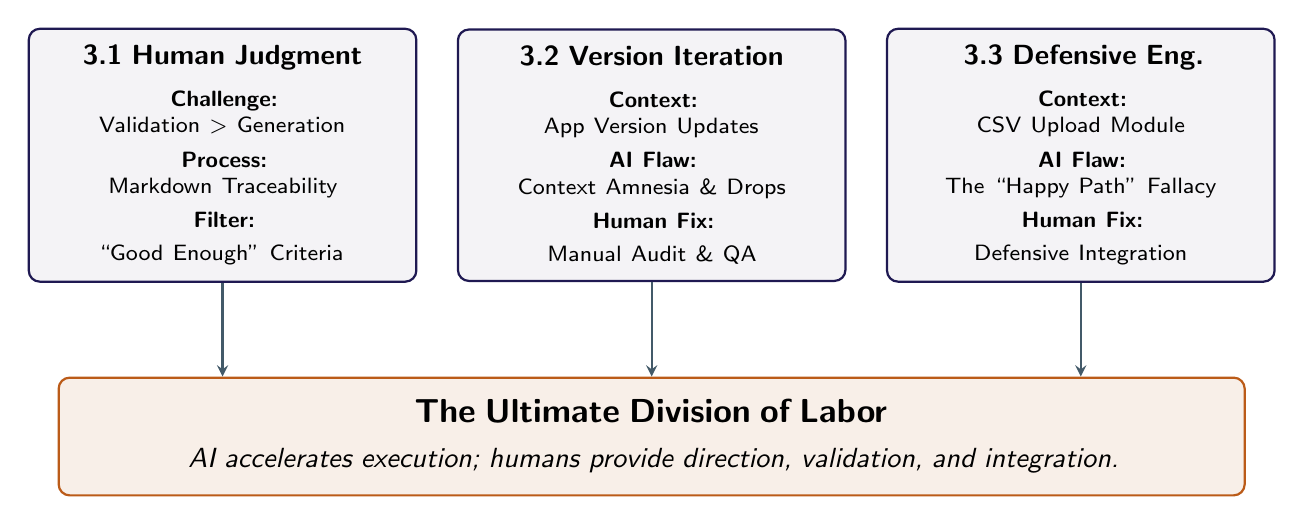
\begin{tikzpicture}[
    node distance=0.6cm and 0.5cm,
    box/.style={draw=primarycolor, thick, rounded corners, align=center, inner sep=6pt, fill=primarycolor!5, text width=4.5cm, minimum height=2.8cm},
    conclusion/.style={draw=accentcolor, thick, rounded corners, align=center, inner sep=8pt, fill=accentcolor!10, text width=14.5cm},
    arrow/.style={->, thick, draw=aaugray, >=stealth}
]

% Pillar 1: 3.1
\node[box] (b1) {
    \textbf{3.1 Human Judgment}\\[0.2cm]
    \footnotesize \textbf{Challenge:}\\ Validation $>$ Generation\\[0.1cm]
    \footnotesize \textbf{Process:}\\ Markdown Traceability\\[0.1cm]
    \footnotesize \textbf{Filter:}\\ ``Good Enough'' Criteria
};

% % Pillar 2: 3.2
% \node[box, right=of b1] (b2) {
%     \textbf{3.2 Systems Thinking}\\[0.2cm]
%     \footnotesize \textbf{Context:}\\ Cloud Deployment Crash\\[0.1cm]
%     \footnotesize \textbf{AI Flaw:}\\ Local Patching (Symptom)\\[0.1cm]
%     \footnotesize \textbf{Human Fix:}\\ Root Cause Defense
% };

% Pillar 2: 3.2
\node[box, right=of b1] (b2) {
    \textbf{3.2 Version Iteration}\\[0.2cm]
    \footnotesize \textbf{Context:}\\ App Version Updates\\[0.1cm]
    \footnotesize \textbf{AI Flaw:}\\ Context Amnesia \& Drops\\[0.1cm]
    \footnotesize \textbf{Human Fix:}\\ Manual Audit \& QA
};

% Pillar 3: 3.3
\node[box, right=of b2] (b3) {
    \textbf{3.3 Defensive Eng.}\\[0.2cm]
    \footnotesize \textbf{Context:}\\ CSV Upload Module\\[0.1cm]
    \footnotesize \textbf{AI Flaw:}\\ The ``Happy Path'' Fallacy\\[0.1cm]
    \footnotesize \textbf{Human Fix:}\\ Defensive Integration
};

% Conclusion Block
\node[conclusion, below=1.2cm of b2] (conc) {
    \textbf{\large The Ultimate Division of Labor}\\[0.15cm]
    \textit{AI accelerates execution; humans provide direction, validation, and integration.}
};

% Connecting Arrows
\draw[arrow] (b1.south) -- (b1.south |- conc.north);
\draw[arrow] (b2.south) -- (conc.north);
\draw[arrow] (b3.south) -- (b3.south |- conc.north);

\end{tikzpicture}
\caption{Logical framework of Human-AI collaboration during system development.}
\label{fig:ai_reflection_summary}
\end{figure}
% --- 图表结束 ---

% ============================================================
% 04_theory.tex
% Section 4: Theoretical Reflection
% ============================================================

\section{Theoretical Reflection}\label{sec:theory}

Taken together, the theories discussed in this section explain the same challenge from different levels of analysis. The jagged frontier highlights the uneven capabilities of AI systems, knowledge codification explains how expertise is embedded into digital artifacts, and augmentation theory clarifies the continuing role of human judgment. Building on these foundations, the TOE framework helps explain why technically feasible systems still struggle to achieve organizational adoption. Together, they suggest that successful digital innovation depends not only on technical capability, but also on the organizational conditions required for adoption.

\subsection{AI and Work: Augmentation, Automation, and the Jagged Frontier}

\subsubsection{The Jagged Frontier in Practice}

Dell'Acqua et al.\parencite{DellAcqua2026} introduce the ``jagged technological frontier'' to describe how AI assistance improves performance on some tasks while degrading it on others, even within the same knowledge workflow and at similar perceived difficulty. Our build process provides a practical example of navigating this frontier.

\textbf{Inside the frontier} (AI helped):
\begin{itemize}
\item Boilerplate Python class definitions, docstrings, and type hints.
\item LaTeX equation formatting and notation tables.
\item Multi-language UI translation (200+ terms from Chinese to pharmaceutical-logistics English).
\item CSS animation and responsive layout code.
\end{itemize}

\textbf{Outside the frontier} (AI harmed or misled):
\begin{itemize}
\item Dependency management for Cloud deployment: the AI added \texttt{torchvision} to solve a symptom rather than the root cause.
\item Reward-function tuning: an initial $\alpha_{\text{setup}} = 5.0$ generated excessive small waves, a behavioral issue the AI failed to recognize.
\item Product positioning: the AI consistently expanded feature scope (NSGA-II, federated learning, 3D visualization) without evaluating whether users actually needed these additions.
\end{itemize}

The last point echoes Shipper's argument in ``After Automation''\parencite{shipper2026after}: as AI commoditizes codified expertise, the value of human judgment increases. While the AI could generate features rapidly, deciding which features created meaningful user value remained a fundamentally human task.

\subsubsection{Knowledge Codification and Its Risks}

Jurowetzki\parencite{Jurowetzki2026}, building on Cowan et al.\parencite{cowan2000codification}, decomposes codification into four capacities: encoding, evaluation, maintenance, and revision. AI dramatically lowers encoding costs by generating code and documentation, but it often increases maintenance and revision challenges.

Consider our \texttt{requirements.txt}. The AI encoded dependencies quickly. However, when the deployment environment changed---through updates to \texttt{transformers}, dependency conflicts, or Streamlit Cloud behavior---the responsibility for evaluating and revising the encoded knowledge fell entirely to the human developer.

This generates what Jurowetzki calls \textbf{orphaned codification}: artifacts whose assumptions are difficult to trace or challenge. Our project contains thousands of lines of AI-generated code whose underlying logic may become increasingly difficult to maintain as platforms evolve.

\subsubsection{Augmentation vs. Automation}

Raisch and Krakowski\parencite{raisch2021automation} describe the ``automation--augmentation paradox'': AI systems that automate routine tasks often increase demand for higher-level human judgment. Maverick-SORT was deliberately designed as an augmentation tool rather than an automation replacement.

Warehouse managers remain the decision-makers; the system recommends but does not execute. Even the What-If simulator is framed as a decision-support tool rather than an autonomous optimizer. This design limits immediate efficiency gains compared with full automation, but it substantially lowers adoption risk because users retain control and can override recommendations.

\subsection{Adoption and Diffusion: A TOE Framework Perspective}

The Technology--Organization--Environment (TOE) framework provides a useful lens for understanding whether Maverick-SORT can move beyond a prototype and achieve real operational adoption.

\paragraph{Technology.}
Maverick-SORT is designed as a decision-support layer rather than a replacement for existing WMS platforms. While WMS systems excel at transaction processing and execution, they provide limited support for simulation, optimization, and scenario analysis. By remaining standalone and browser-based, the system delivers predictive intelligence without requiring costly modifications to legacy infrastructure.

\paragraph{Organization.}
The key adopter is not the IT department but the Operations Director. Unlike IT managers, whose priority is stability and risk avoidance, operations managers are directly responsible for warehouse performance. The Essential Edition lowers adoption barriers by allowing them to evaluate potential value independently through a zero-deployment What-If environment.

\paragraph{Environment.}
Pharmaceutical logistics operates under strict GSP compliance requirements. Rather than treating regulation as an obstacle, Maverick-SORT uses explainable, knowledge-guided recommendations to align optimization with existing operational rules. Regulatory pressure therefore becomes a driver of adoption rather than a barrier.

\paragraph{The Most Limiting Condition.}
Among all TOE factors, the greatest constraint is organizational champion bandwidth. Operations managers often lack the time, attention, and political capital required to evaluate new technologies. Consequently, adoption depends less on algorithmic performance than on reducing the effort required to explore the solution. The Essential Edition, free trial, and five-minute simulation workflow are all designed to minimize this activation cost.

\subsection{Demo Day as an Adoption Test}

The class Demo Day provided a useful reality check regarding how the system was perceived compared with how it was built.

\begin{itemize}
\item \textbf{What resonated most (System Logic).} Reviewers were most engaged by the relationships between components---particularly how KGDRL recommendations connected to the Algorithm Arena and AI Copilot explanations.

```
\item \textbf{What was largely ignored (Visual Complexity).} Detailed dashboard visualizations attracted relatively little attention. Without sufficient operational context, many charts appeared as generic analytics rather than sources of business value.

\item \textbf{The core skepticism (Product Identity).} The strongest critiques questioned the product's fundamental value proposition: \textit{What is the core benefit? Why would someone adopt this system?}
```

\end{itemize}

\textbf{The Key Lesson.} This feedback revealed that my immediate challenge was not technical performance but narrative clarity. As a result, we shifted the project's positioning away from a feature-oriented demonstration and toward the concept of a ``Risk Reversal Engine'' designed to reduce adoption friction. The experience reinforced the broader conclusion of this report: organizational attention, rather than algorithm quality, is often the primary constraint on digital innovation adoption.


\section{Results, Limitations, and Further Opportunities}
\label{sec:results}

\subsection{What We Validated}

\begin{enumerate}
\item \textbf{The concept is technically viable.} The KGDRL architecture successfully generated feasible scheduling recommendations and supported scenario-based decision making, demonstrating that AI-assisted wave allocation can be implemented within a lightweight prototype.

\item \textbf{Reducing perceived risk matters more than improving performance.} In informal testing with supply-chain classmates, the What-If simulator generated significantly more interest than benchmark results alone. Users were more willing to explore the system when they could safely experiment with scenarios before committing to adoption.

\end{enumerate}

\subsection{An Unexpected Finding}

One unexpected lesson was that increasing algorithmic sophistication did not automatically increase perceived value. Discussions during development and Demo Day focused far more on deployment effort, explainability, and integration concerns than on optimization performance. This reinforced our central insight that organizational attention, rather than algorithm quality, represents the primary constraint on adoption.

\subsection{Current Limitations}

\begin{enumerate}
\item \textbf{Prototype-level infrastructure.} Streamlit enabled rapid development but lacks the responsiveness and scalability expected in a production warehouse environment.

\item \textbf{Simplified operational assumptions.} The reward function captures key scheduling objectives but omits real-world factors such as picker fatigue, equipment congestion, and organizational coordination.

\item \textbf{Limited interactivity.} Several modules remain demonstration-oriented rather than fully interactive, restricting their usefulness for continuous decision support.


\end{enumerate}

\subsection{Next Step}

The next step is not further algorithm validation, but adoption validation. A four-week pilot in a real warehouse would allow observation of whether managers regularly use the system, trust its recommendations, and integrate it into daily decision-making. Such evidence would directly test whether organizational attention is indeed the primary barrier to adoption.

The central lesson of Maverick-SORT is that creating a technically capable AI system is only part of the innovation challenge. Real impact depends on whether potential users can understand, evaluate, and trust that system within the constraints of their everyday work.

% ── References ───────────────────────────────────────────────
% Printed here. Does not count toward the 10-page limit.
\newpage
\printbibliography[heading=bibintoc, title={References}]

% ── AI-use declaration ───────────────────────────────────────
% Required. Does not count toward the 10-page limit.
\newpage
\section{AI-Use Declaration}
\addcontentsline{toc}{section}{AI-Use Declaration}

This document was prepared with assistance from Claude Code (Anthropic CLI) using an API service provided through Kimi/Moonshot. Consistent with the course's view of AI as an accountable collaborator rather than a black box, this declaration clarifies how AI was used in producing the report itself, separate from the development of Maverick-SORT.

\begin{itemize}
\item \textbf{Content Extraction and Synthesis}: Development logs, including the continuously updated \textit{AI\_Tools\_Usage\_Review.md}, were provided to the AI as reference material. The AI assisted in extracting project milestones, technical decisions, and implementation details to support the narrative structure of this report.

\item \textbf{Human-Led Research Design}: The human author retained responsibility for all conceptual and methodological decisions, including the mathematical formulation, reinforcement-learning design choices, reward-function specification, parameter calibration, and experimental design. AI tools occasionally assisted with implementation and debugging, but they did not determine the underlying research logic.

\item \textbf{Drafting and Formatting Support}: The AI assisted with LaTeX formatting, structural organization, language refinement, and the preparation of early drafts based on detailed human instructions and outlines.

\end{itemize}

AI assistance proved highly effective for drafting, formatting, translation, and code scaffolding. However, tasks involving system design, product positioning, theoretical interpretation, and experimental judgment remained primarily human-led. This pattern is consistent with the ``jagged frontier'' discussed in Section~\ref{sec:theory}.

Consistent with the course's emphasis on accountable AI use, the human author remained responsible for evaluating outputs, verifying technical claims, making design decisions, and determining the final arguments presented in this report. All errors, interpretations, and conclusions remain the responsibility of the author.


% ── Appendices ───────────────────────────────────────────────
% Architecture diagram and screenshots.
% Does not count toward the 10-page limit.
\newpage
% ============================================================
% appendix.tex
% Appendices: Architecture Diagram and Screenshots
% ============================================================

\appendix
\section{Product Architecture}
\label{app:architecture}

\begin{figure}[htbp]
\centering
\fbox{\parbox{0.9\textwidth}{
\centering
\vspace{0.3cm}
\textbf{Maverick-SORT Essential Architecture}
\vspace{0.2cm}

\texttt{orders.csv .etc} / demo data
$\rightarrow$ \texttt{DataGenerator} / upload router
$\rightarrow$ \texttt{PharmaWaveEnv} (MDP environment)
$\rightarrow$ \texttt{KnowledgeGuidedPPO} (GAT + PPO + KL)
$\rightarrow$ \texttt{WhatIfSimulator} (scenario comparison)
$\rightarrow$ \texttt{Streamlit Dashboard} (Algorithm Arena + visualizations)

\vspace{0.3cm}
}}
\caption{Simplified system architecture. Solid lines indicate data flow; dashed lines indicate optional LLM explanations via Hugging Face.}
\label{fig:arch}
\end{figure}


\section{Key Screenshots}
\label{app:screenshots}

\textit{Note: The following screenshots are placeholders for the final submission. High-resolution versions will be included in the PDF appendix.}

\begin{enumerate}
    \item \textbf{Algorithm Arena}: Comparison of KGDRL vs. baselines on reward, picking distance, and temperature violations.
    \item \textbf{What-If Scenario Simulator}: Parameter sweep showing cost sensitivity to wave capacity changes.
    \item \textbf{Real-Time Simulation}: Streamlit dashboard displaying wave composition, zone coverage, and compliance status.
\end{enumerate}


\section{PPO Hyperparameters}
\label{app:hyperparams}

\begin{table}[htbp]
\centering
\caption{Final PPO Hyperparameters}
\begin{tabular}{ll}
\hline
Parameter & Value \\
\hline
Actor learning rate & $5 \times 10^{-4}$ \\
Critic learning rate & $1 \times 10^{-5}$ \\
Discount factor $\gamma$ & 0.96 \\
GAE lambda & 0.95 \\
PPO clip $\epsilon$ & 0.2 \\
Hidden dimension & 128 \\
Training episodes & 120 \\
KL constraint weight $\lambda_{\text{kg}}$ & 0.1 \\
\hline
\end{tabular}
\end{table}


% ============================================================
\end{document}
% ============================================================

% ── Template credit ──────────────────────────────────────────
% Digital Innovation · SDC / AAUBS / UCAS · 2026
% Template: Eskil Olav Andersen, Aalborg University Business School
